%\VignetteIndexEntry{The qsmooth user's guide}
%\VignettePackage{qlasso}
%\VignetteEngine{knitr::knitr}
\documentclass{article}\usepackage[]{graphicx}\usepackage[usenames,dvipsnames]{color}
%% maxwidth is the original width if it is less than linewidth
%% otherwise use linewidth (to make sure the graphics do not exceed the margin)
\makeatletter
\def\maxwidth{ %
  \ifdim\Gin@nat@width>\linewidth
    \linewidth
  \else
    \Gin@nat@width
  \fi
}
\makeatother

\definecolor{fgcolor}{rgb}{0.345, 0.345, 0.345}
\newcommand{\hlnum}[1]{\textcolor[rgb]{0.686,0.059,0.569}{#1}}%
\newcommand{\hlstr}[1]{\textcolor[rgb]{0.192,0.494,0.8}{#1}}%
\newcommand{\hlcom}[1]{\textcolor[rgb]{0.678,0.584,0.686}{\textit{#1}}}%
\newcommand{\hlopt}[1]{\textcolor[rgb]{0,0,0}{#1}}%
\newcommand{\hlstd}[1]{\textcolor[rgb]{0.345,0.345,0.345}{#1}}%
\newcommand{\hlkwa}[1]{\textcolor[rgb]{0.161,0.373,0.58}{\textbf{#1}}}%
\newcommand{\hlkwb}[1]{\textcolor[rgb]{0.69,0.353,0.396}{#1}}%
\newcommand{\hlkwc}[1]{\textcolor[rgb]{0.333,0.667,0.333}{#1}}%
\newcommand{\hlkwd}[1]{\textcolor[rgb]{0.737,0.353,0.396}{\textbf{#1}}}%

\usepackage{framed}
\makeatletter
\newenvironment{kframe}{%
 \def\at@end@of@kframe{}%
 \ifinner\ifhmode%
  \def\at@end@of@kframe{\end{minipage}}%
  \begin{minipage}{\columnwidth}%
 \fi\fi%
 \def\FrameCommand##1{\hskip\@totalleftmargin \hskip-\fboxsep
 \colorbox{shadecolor}{##1}\hskip-\fboxsep
     % There is no \\@totalrightmargin, so:
     \hskip-\linewidth \hskip-\@totalleftmargin \hskip\columnwidth}%
 \MakeFramed {\advance\hsize-\width
   \@totalleftmargin\z@ \linewidth\hsize
   \@setminipage}}%
 {\par\unskip\endMakeFramed%
 \at@end@of@kframe}
\makeatother

\definecolor{shadecolor}{rgb}{.97, .97, .97}
\definecolor{messagecolor}{rgb}{0, 0, 0}
\definecolor{warningcolor}{rgb}{1, 0, 1}
\definecolor{errorcolor}{rgb}{1, 0, 0}
\newenvironment{knitrout}{}{} % an empty environment to be redefined in TeX

\usepackage{alltt}

\RequirePackage{/Library/Frameworks/R.framework/Versions/3.1/Resources/library/BiocStyle/resources/latex/Bioconductor}

\AtBeginDocument{\bibliographystyle{/Library/Frameworks/R.framework/Versions/3.1/Resources/library/BiocStyle/resources/latex/unsrturl}}


\setlength{\parskip}{1\baselineskip}
\setlength{\parindent}{0pt}

\title{The \texttt{qsmooth} user's guide}
\author{Kwame Okrah \texttt{kwame.okrah@gmail.com} \and
Hector Corrado Bravo \texttt{hcorrada@gmail.com} \and
Stephanie C. Hicks \texttt{shicks@jimmy.harvard.edu} \and
Rafael A. Irizarry \texttt{rafa@jimmy.harvard.edu} }

\date{Modified: March 5, 2015.  Compiled: \today}
\IfFileExists{upquote.sty}{\usepackage{upquote}}{}
\begin{document}

\maketitle
 
\tableofcontents

\section{Introduction}

Add introduction here. 

\section{Getting Started}

Load the \texttt{qlasso} package in R. 

\begin{knitrout}
\definecolor{shadecolor}{rgb}{0.969, 0.969, 0.969}\color{fgcolor}\begin{kframe}
\begin{alltt}
\hlkwd{library}\hlstd{(quantro)}
\hlkwd{library}\hlstd{(HTShape)}
\hlkwd{library}\hlstd{(qlasso)}
\end{alltt}
\end{kframe}
\end{knitrout}


\section{Data}

\subsection{Pickrell Data Example}
Load an example data set. Here we use the Pickrell data set. 
(but we can change this to whatever). 

\begin{knitrout}
\definecolor{shadecolor}{rgb}{0.969, 0.969, 0.969}\color{fgcolor}\begin{kframe}
\begin{alltt}
\hlkwd{data}\hlstd{(examplesData)}
\hlkwd{names}\hlstd{(examplesData)}
\end{alltt}
\begin{verbatim}
## [1] "bottomly"            "pickrell"            "tcruziExtracellular"
## [4] "seqc"                "seqc.ercc"
\end{verbatim}
\begin{alltt}
\hlstd{counts} \hlkwb{=} \hlstd{examplesData}\hlopt{$}\hlstd{pickrell}\hlopt{$}\hlstd{exprs}
\hlstd{groups} \hlkwb{=} \hlstd{examplesData}\hlopt{$}\hlstd{pickrell}\hlopt{$}\hlstd{cond}
\end{alltt}
\end{kframe}
\end{knitrout}

\section{Exploratory Data Analysis}

In this section we will look at summary plots
of the raw data.

% 
% <<librarysize, fig.width=4.5, fig.height=2.5, fig.align='center', echo=FALSE>>=
%  par(mgp=c(1.5, 0.5, 0), mar=c(2.5, 2.5, 1, 0.5))
%  
%  groupCol = ifelse(groups=="female", "steelblue", "tomato")
%  
%  barplot(colSums(counts), col=groupCol, main="Library size",
%          xaxt="none", xlab="Samples", ylab="Reads aligned")
% @

First, we will filter out genes with low counts with the \texttt{filterCounts}
function. This function will only retain genes whose counts per million (cpm)
exceeds 1 (can be changed, see the \texttt{thresh} parameter) in a given
number of samples (see the \texttt{minSamples} parameter).

\begin{knitrout}
\definecolor{shadecolor}{rgb}{0.969, 0.969, 0.969}\color{fgcolor}\begin{kframe}
\begin{alltt}
\hlstd{(minSamples} \hlkwb{<-} \hlkwd{min}\hlstd{(}\hlkwd{table}\hlstd{(groups)))}
\end{alltt}
\begin{verbatim}
## [1] 29
\end{verbatim}
\begin{alltt}
\hlkwd{dim}\hlstd{(counts)}
\end{alltt}
\begin{verbatim}
## [1] 38415    69
\end{verbatim}
\begin{alltt}
\hlstd{counts} \hlkwb{=} \hlkwd{filterCounts}\hlstd{(counts,} \hlkwc{thresh}\hlstd{=}\hlnum{1}\hlstd{,} \hlkwc{minSamples}\hlstd{=minSamples)}
\hlkwd{dim}\hlstd{(counts)}
\end{alltt}
\begin{verbatim}
## [1] 17471    69
\end{verbatim}
\end{kframe}
\end{knitrout}

Density plots.
\begin{knitrout}
\definecolor{shadecolor}{rgb}{0.969, 0.969, 0.969}\color{fgcolor}

{\centering 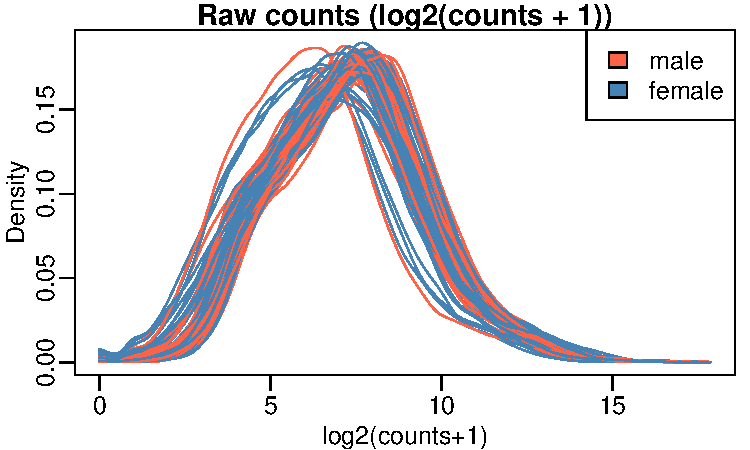
\includegraphics[width=\maxwidth]{figure/density-1} 

}



\end{knitrout}

\subsection{Samples shape assessment}

In this section we will formally test whether the transcriptome
shapes (densities) differ due to a factor of interest. In this case
sex. We will use both quantro and HTShape for this test and compare results.

\subsubsection{L-ratios manova stat.}

First we will use the \texttt{shapeManova} function in HTShape 
(see HTShape for more details). This method first summarizes each
sample in the data set with scale-free skewness and kurtosis coefficients
(L-skew and L-kurt). These shape esitmates are based on the theory of L-moments 
(cite:Hosking1990, Okrah2015). We perform a multivariate analysis of 
variance based on the shape (L-skew, L-kurt) esitmates
(see xxx for more details).

\begin{knitrout}
\definecolor{shadecolor}{rgb}{0.969, 0.969, 0.969}\color{fgcolor}

{\centering 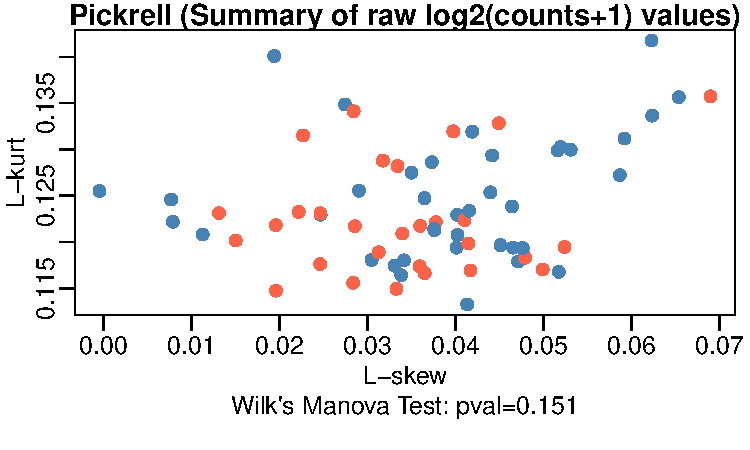
\includegraphics[width=\maxwidth]{figure/lrats-1} 

}


\begin{kframe}\begin{verbatim}
## $WL
## [1] 0.9451745
## 
## $Fstat
## [1] 1.887206
## 
## $df1
## [1] 2
## 
## $df2
## [1] 132
## 
## $pval
## [1] 0.1512349
\end{verbatim}
\end{kframe}
\end{knitrout}

The pvalue of 0.151 indicates that sex and transcriptome shape are not
related.

\subsubsection{Quantro stat.}

Use qauntro for the same test. 

\begin{knitrout}
\definecolor{shadecolor}{rgb}{0.969, 0.969, 0.969}\color{fgcolor}\begin{kframe}
\begin{alltt}
\hlstd{(qtest} \hlkwb{<-} \hlkwd{quantro}\hlstd{(}\hlkwd{log2}\hlstd{(counts}\hlopt{+}\hlnum{1}\hlstd{), groups,} \hlkwc{verbose}\hlstd{=}\hlnum{FALSE}\hlstd{,} \hlkwc{B}\hlstd{=}\hlnum{500}\hlstd{))}
\end{alltt}
\begin{verbatim}
## quantro: Test for global differences in distributions
##    nGroups:  2 
##    nTotSamples:  69 
##    nSamplesinGroups:  40 29 
##    anovaPval:  0.50626 
##    quantroStat:  2.01579 
##    quantroPvalPerm:  0.094
\end{verbatim}
\end{kframe}
\end{knitrout}

Conclusions are the same as shapeManova. 

\section{Using \texttt{qlasso} for normalization}

\subsection{Scale samples}
Scale samples using trimmed mean. Trim off top and bottom 0.25 quantiles.
Other methods can be used (eg. AH, median, mean).

Density plots
\begin{knitrout}
\definecolor{shadecolor}{rgb}{0.969, 0.969, 0.969}\color{fgcolor}

{\centering 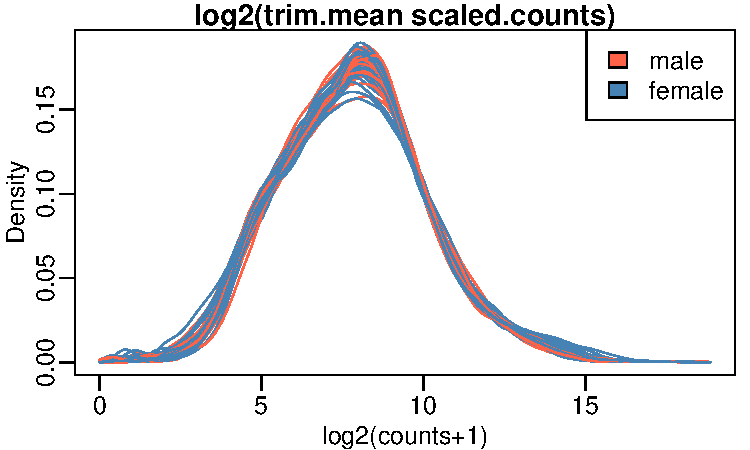
\includegraphics[width=\maxwidth]{figure/scale-counts-1} 

}



\end{knitrout}


\subsection{Computing quantiles}

The sample quantiles of the raw data, reference quantile, 
and shrinkage weights can be computed using the 
\texttt{qstats()} function. The reference quantile 
can be computed as a average across sample quantiles 
(as in full quantile normalization) or can be obtained
by taking the median across reference quantiles. 
The \texttt{refType} parameter specifies which type
of reference quantile to use.

\begin{knitrout}
\definecolor{shadecolor}{rgb}{0.969, 0.969, 0.969}\color{fgcolor}\begin{kframe}
\begin{alltt}
\hlstd{qs} \hlkwb{=} \hlkwd{qstats}\hlstd{(}\hlkwc{exprs}\hlstd{=}\hlkwd{log2}\hlstd{(scaled.counts),} \hlkwc{groups}\hlstd{=groups,}
            \hlkwc{refType}\hlstd{=}\hlstr{"mean"}\hlstd{,} \hlkwc{groupLoc}\hlstd{=}\hlstr{"mean"}\hlstd{,} \hlkwc{window}\hlstd{=}\hlnum{99}\hlstd{)}
\end{alltt}
\end{kframe}
\end{knitrout}

plots weights
\begin{knitrout}
\definecolor{shadecolor}{rgb}{0.969, 0.969, 0.969}\color{fgcolor}

{\centering 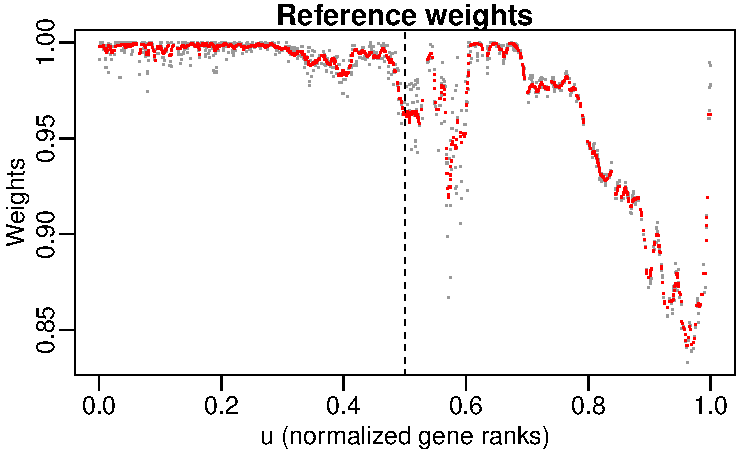
\includegraphics[width=\maxwidth]{figure/weights-1} 

}



\end{knitrout}


\subsection{\texttt{qshrink} normalized values}

The normalized values are computed using the 
\texttt{qshrink} function. 
This function is based on the resultys of \texttt{qstats}.
We do not need to call \texttt{qstats}. It was shown 
above for demonstration.

\begin{knitrout}
\definecolor{shadecolor}{rgb}{0.969, 0.969, 0.969}\color{fgcolor}

{\centering 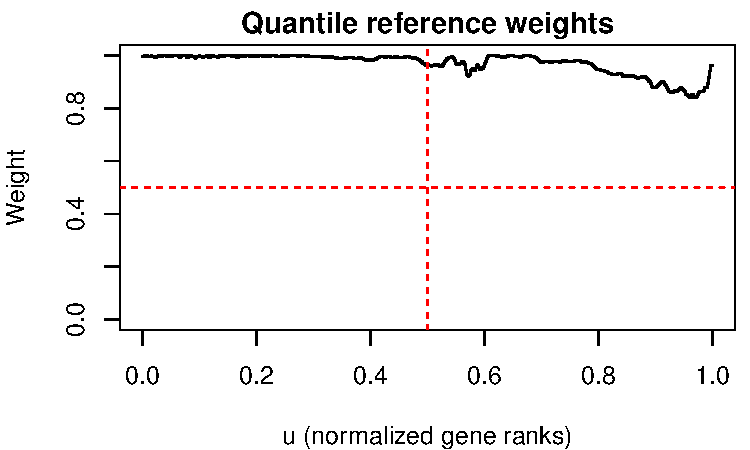
\includegraphics[width=\maxwidth]{figure/qshrikage-1} 

}



\end{knitrout}
The weights in this plot are the same as the weights above. 
(final vignette will not include above plot.)

Boxplots
\begin{knitrout}
\definecolor{shadecolor}{rgb}{0.969, 0.969, 0.969}\color{fgcolor}

{\centering 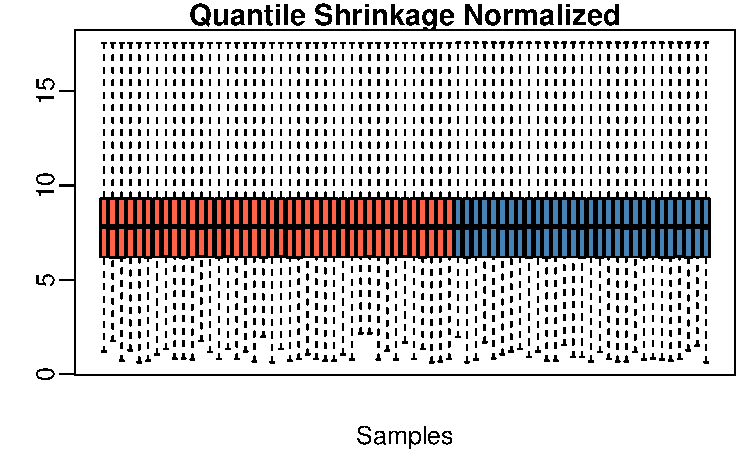
\includegraphics[width=\maxwidth]{figure/boxplots-normExprs-1} 

}



\end{knitrout}

Density plots
\begin{knitrout}
\definecolor{shadecolor}{rgb}{0.969, 0.969, 0.969}\color{fgcolor}

{\centering 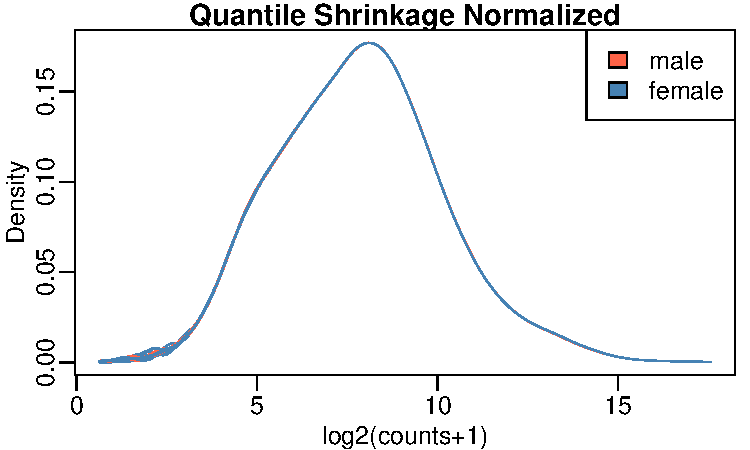
\includegraphics[width=\maxwidth]{figure/density-normExprs-1} 

}



\end{knitrout}


\section{SessionInfo}

\begin{knitrout}
\definecolor{shadecolor}{rgb}{0.969, 0.969, 0.969}\color{fgcolor}\begin{kframe}
\begin{alltt}
\hlkwd{sessionInfo}\hlstd{()}
\end{alltt}
\begin{verbatim}
## R version 3.1.2 (2014-10-31)
## Platform: x86_64-apple-darwin10.8.0 (64-bit)
## 
## locale:
## [1] en_US.UTF-8/en_US.UTF-8/en_US.UTF-8/C/en_US.UTF-8/en_US.UTF-8
## 
## attached base packages:
## [1] stats     graphics  grDevices utils     datasets  methods   base     
## 
## other attached packages:
## [1] qlasso_0.0.0.9000 HTShape_1.0.0     quantro_1.0.0     knitr_1.9        
## 
## loaded via a namespace (and not attached):
##  [1] annotate_1.44.0       AnnotationDbi_1.28.2  base64_1.1           
##  [4] beanplot_1.2          Biobase_2.26.0        BiocGenerics_0.12.1  
##  [7] BiocStyle_1.4.1       Biostrings_2.34.1     bumphunter_1.6.0     
## [10] codetools_0.2-11      colorspace_1.2-6      compiler_3.1.2       
## [13] DBI_0.3.1             digest_0.6.8          doParallel_1.0.8     
## [16] doRNG_1.6             evaluate_0.6          foreach_1.4.2        
## [19] formatR_1.1           genefilter_1.48.1     GenomeInfoDb_1.2.5   
## [22] GenomicRanges_1.18.4  ggplot2_1.0.1         grid_3.1.2           
## [25] gtable_0.1.2          highr_0.4.1           illuminaio_0.8.0     
## [28] IRanges_2.0.1         iterators_1.0.7       lattice_0.20-31      
## [31] limma_3.22.7          locfit_1.5-9.1        MASS_7.3-40          
## [34] matrixStats_0.14.0    mclust_5.0.0          minfi_1.12.0         
## [37] multtest_2.22.0       munsell_0.4.2         nlme_3.1-120         
## [40] nor1mix_1.2-0         parallel_3.1.2        pkgmaker_0.22        
## [43] plyr_1.8.1            preprocessCore_1.28.0 proto_0.3-10         
## [46] quadprog_1.5-5        RColorBrewer_1.1-2    Rcpp_0.11.5          
## [49] registry_0.2          reshape_0.8.5         reshape2_1.4.1       
## [52] rngtools_1.2.4        RSQLite_1.0.0         S4Vectors_0.4.0      
## [55] scales_0.2.4          siggenes_1.40.0       splines_3.1.2        
## [58] stats4_3.1.2          stringr_0.6.2         survival_2.38-1      
## [61] tools_3.1.2           XML_3.98-1.1          xtable_1.7-4         
## [64] XVector_0.6.0         zlibbioc_1.12.0
\end{verbatim}
\end{kframe}
\end{knitrout}


\end{document}
